\documentclass[10pt,twocolumn]{article}
\usepackage[margin=0.62in,columnsep=0.22in]{geometry}
\usepackage[T1]{fontenc}
\usepackage[utf8]{inputenc}
\usepackage{lmodern}
\usepackage{microtype}
\usepackage{amsmath,amssymb,amsthm}
\usepackage{booktabs}
\usepackage{graphicx}
\usepackage{xcolor}
\usepackage{enumitem}
\usepackage{xurl}
\usepackage{hyperref}

\hypersetup{
  colorlinks=true,
  linkcolor=blue!60!black,
  citecolor=blue!60!black,
  urlcolor=blue!60!black,
  pdftitle={Constructive Lean 4 Kernel and Exact Zero-Float Certificates for OpenAI Superpolynomial Simple Polytope Diameter},
  pdfauthor={Lluis Eriksson}
}

\newtheorem{proposition}{Proposition}
\newtheorem{definition}{Definition}
\newcommand{\ZZ}{\mathbb{Z}}
\newcommand{\NN}{\mathbb{N}}
\newcommand{\QQ}{\mathbb{Q}}
\newcommand{\RR}{\mathbb{R}}

\title{\vspace{-0.9em}\textbf{Constructive Lean~4 Kernel and Exact Zero-Float Certificates for OpenAI's Superpolynomial Simple Polytope Diameter}}
\author{Lluis Eriksson\thanks{Independent Researcher. Code, Lean~4 proofs, and certificates: MIT License; manuscript and figures: CC-BY-4.0. Prepared with transparent AI coding, formalization, and drafting assistance via Google Antigravity; all Lean~4 theorems, exact zero-float verifiers, and adversarial tests were independently compiled and verified locally. Repository: \href{https://github.com/lluiseriksson/openai-simple-polytope-diameter-certificates}{\nolinkurl{github.com/lluiseriksson/openai-simple-polytope-diameter-certificates}}.}}
\date{November 25, 2026}

\begin{document}
\maketitle
\vspace{-1.2em}

\begin{abstract}
A November~24, 2026 companion preprint from OpenAI~\cite{openai2026hirsch} proposes a disproof of the polynomial Hirsch conjecture by constructing rational simple $d$-polytopes with $n$ facets whose graph diameter (and even subpolynomial $s(d)$-dimensional face-move distance) exceeds every polynomial in $n$, alongside corollaries for complementary $2d$-facet polytopes, Minkowski sums of two simplices, Schlegel regular triangulations, and symmetric positive doubly-stochastic packing linear programs. Rather than assuming peer-reviewed endorsement of its hierarchical scheduler, blocking-module, or recursive substitution machinery, we deliver an independent, explicitly scoped, zero-floating-point verification companion for its discrete convex-corner bend, prescribed dimension/facet product padding, Klee--Walkup wedge complementary-tip lifting, Schlegel projective prismatoid and middle-section lifting, and two-stage symmetric doubly-stochastic packing mechanisms. Layer~1 (\texttt{OpenAI\allowbreak HirschDiameter.lean}) proves 18 standalone constructive Lean~4.35.0 geometric and algebraic sub-lemmas (zero \texttt{sorry}, zero \texttt{axiom}, zero \texttt{Classical.choice}, zero warnings; 1 \texttt{none}, 1 \texttt{[propext]}, and 16 \texttt{[propext, Quot.sound]}). Layer~2 (\texttt{HIRSCH-DIAM-CERT-1.0}) is a pure-stdlib Python \texttt{int}/\texttt{Fraction} 4-mode auditor certifying 16 canonical finite witnesses in $0.092$--$19.354\,\mathrm{ms}$ and rejecting 76/76 live adversarial forgeries with exact branch assertions (82/82 pytest checks).
\end{abstract}

\section{Introduction and Scope Calibration}\label{sec:intro}
The Hirsch conjecture (1957; see~\cite{dantzig1963linear,klee1967dstep}) predicted that every $d$-polytope with $n$ facets has edge-graph diameter at most $n-d$. Santos~\cite{santos2012counterexample} refuted the linear bound via a 43-dimensional, 86-facet polytope of diameter at least $44 > 86-43$, while Kalai--Kleitman~\cite{kalai1992quasi}, Todd~\cite{todd2014improved}, and Sukegawa~\cite{sukegawa2019asymptotically} proved quasi-polynomial upper bounds $n^{\log_2 d + O(1)}$. Whether a \emph{polynomial} diameter bound $\mathrm{poly}(n,d)$ holds remained open. OpenAI's November~24, 2026 companion preprint~\cite{openai2026hirsch} proposes a disproof of the polynomial Hirsch conjecture (Theorems~1.1--1.2) together with three explicit geometric/LP corollaries built from four verifiable discrete-algebraic mechanisms:
\begin{enumerate}[leftmargin=1.2em,itemsep=1pt,topsep=2pt]
  \item \textbf{Convex Corner Bends, Crossing Bounds \& Product Padding (Secs.~1.2, 2.1--2.2, Lem.~2.2, Thm.~1.2):} An affine segment cannot cross a V-corner $z\ge |x-a|$ with $z(a)=0$ without bending (slope jump $\ge 2$); Lemma~2.2 gives exact crossing bounds $R N^K$ and $R N^{K-1}\max(0, Ng-8)$, while Theorem~1.2 pads any $(d_0,f_0)$ seed with a $(d-d_0-2)$-simplex and $(E+d_0-f_0+1)$-gon to hit exact $(d,d+E)$.
  \item \textbf{Klee--Walkup Wedge to Complementary $2d$-Facet Polytopes (Sec.~14, Cor.~14.1):} Applying $m-2p$ Klee--Walkup wedges~\cite{klee1967dstep} on facets uncovered by disjoint tips $v,w$ yields a rational simple $(m-p)$-polytope with exactly $2(m-p)$ facets and complementary lifted tips.
  \item \textbf{Schlegel Projective Lifting \& Prismatoid Middle Section (Sec.~14.1, Cor.~14.2):} Slicing a simplicial prismatoid $\mathrm{conv}((U,0)\cup(V,1))$ at height $1/2$ yields $(U+V)/2$ with $\le d^2$ pairwise vertex sums and facet distance $D_s - 2$, while $(X,Z)=(\frac{x}{1+z},\frac{-z}{1+z})$ transforms every non-base facet $a\cdot x + b z\le c$ ($b+c>0$) to $a\cdot X - (b+c)Z \le c$~\cite{ziegler1995lectures}, yielding Schlegel triangulation depth $D_s-1$.
  \item \textbf{Two-Stage Symmetric Positive Doubly-Stochastic Packing LP (Sec.~14.2, Cor.~14.3):} Starting from an invertible nonnegative $k\times k$ packing $Ax\le 1$ ($A\mathbf{1}=\mathbf{1}$), Stage~1 forms $B_0=(A+\mathbf{1}c^\top)/h$ with exact projective bijection $y=\frac{hx}{1+c^\top x}$ preserving slack $1-B_0y=\frac{1-Ax}{1+c^\top x}$, and Stage~2 forms symmetric doubly-stochastic $B=(H+t\mathbf{1}\mathbf{1}^\top)/(1+dt)$ with $\max_{i,j}|B_{ij}-1/d|<\epsilon$.
\end{enumerate}

\paragraph{Honest Two-Layer Verification Scope.}
\begin{enumerate}[leftmargin=1.2em,itemsep=1pt,topsep=2pt]
  \item \textbf{Layer~1 (Lean~4.35.0 Kernel, Standalone Sub-Lemmas):} \texttt{lean/OpenAI\allowbreak HirschDiameter.lean} proves 18 standalone constructive geometric and algebraic sub-lemmas (Table~\ref{tab:lean18}) extracted from Sections~1, 1.2, 2.1, 2.2, 13.5, 14, 14.1, and~14.2 of~\cite{openai2026hirsch}.
  \item \textbf{Layer~2 (Exact Zero-Float Auditor):} \texttt{HIRSCH-\allowbreak DIAM-\allowbreak CERT-1.0} audits 16 canonical finite witnesses across V-corner zigzag paths, Lemma~2.2 / Theorem~1.2 accounting, exact bounded irredundant Klee--Walkup wedges with full vertex-lattice enumeration ($d\le 5$), exact complete Schlegel projective prismatoids with exact dual-graph BFS width ($d\le 5$, $D_1\in\{2,3,4,5\}$), and exact two-stage symmetric doubly-stochastic packings ($d\le 9$).
  \item \textbf{Explicit Non-Claims:} We do \emph{not} formalize in Lean~4 the hierarchical scheduler (Sections~3--13), blocking-module tournament constructions, generic perturbation openness arguments, or the full $n^{\omega(1)}$ asymptotic diameter lower bound of Theorems~1.1--1.2; those recursive construction pillars remain unverified outside the companion preprint~\cite{openai2026hirsch}.
\end{enumerate}

\section{Constructive Lean~4.35.0 Kernel}\label{sec:lean}
\texttt{lean/OpenAI\allowbreak HirschDiameter.lean} compiles standalone under Lean~4.35.0~\cite{demoura2021lean4} with zero external imports, zero warnings, zero \texttt{sorry}, and zero \texttt{Classical.choice}. Auditing via \texttt{AuditAxioms.lean} confirms 1 zero-axiom theorem (\texttt{none}: \#3), 1 \texttt{[propext]} theorem (\texttt{P}: \#18), and 16 \texttt{[propext, Quot.sound]} theorems (\texttt{P,Q}; Table~\ref{tab:lean18}).

\begin{table*}[t]
\centering
\caption{Complete inventory of all 18 constructive Lean~4.35.0 sub-lemmas in \texttt{lean/OpenAIHirschDiameter.lean} (zero \texttt{sorry}, zero \texttt{axiom}, zero \texttt{Classical.choice}, zero warnings; \texttt{none} for \#3; \texttt{[propext]} (\texttt{P}) for \#18; \texttt{[propext, Quot.sound]} (\texttt{P,Q}) for the remaining 16).}
\label{tab:lean18}
\scriptsize
\setlength{\tabcolsep}{2.1pt}
\begin{tabular}{@{}r l l p{9.6cm} l@{}}
\toprule
\# & Theorem Identifier & Ref.~\cite{openai2026hirsch} & Exact Machine-Checked Statement \& Hypotheses & Ax. \\
\midrule
1 & \texttt{sec12\_affine\_cannot\_cross\_corner} & Sec.~1.2 & $\forall m,d\in\ZZ,\ 0<d \wedge d\le -(md) \wedge d\le md \implies \mathrm{False}$. & \texttt{P,Q} \\
2 & \texttt{sec12\_corner\_slope\_contradiction} & Sec.~1.2 & $\forall m\in\ZZ,\ m\le -1 \wedge 1\le m \implies \mathrm{False}$. & \texttt{P,Q} \\
3 & \texttt{sec1\_santos\_2012\_hirsch\_violation} & Sec.~1 & $86 - 43 = 43 \wedge 43 < 44$ (Santos 2012 violation~\cite{santos2012counterexample}). & \texttt{none} \\
4 & \texttt{sec12\_recursive\_crossing\_step} & Sec.~1.2 & $\forall N,q,D\in\NN,\ 4\le NqD \implies 1\le \lfloor NqD/4\rfloor$. & \texttt{P,Q} \\
5 & \texttt{lem22\_cell\_distance\_lower\_bound} & Lem.~2.2 & $\forall c,N_g,R,P\in\NN,\ 8+c\le N_g \wedge 1\le RP \implies c\le RP(N_g-8)$. & \texttt{P,Q} \\
6 & \texttt{thm12\_product\_dimension\_exact} & Thm.~1.2 & $\forall d,d_0\in\NN,\ d_0+2\le d \implies d_0+(d-d_0-2)+2 = d$. & \texttt{P,Q} \\
7 & \texttt{thm12\_product\_facets\_exact} & Thm.~1.2 & $\forall d,d_0,E,f\in\NN,\ d_0+2\le d \wedge f\le E+d_0 \implies f+(d-d_0-1)+(E+d_0-f+1)=d+E$. & \texttt{P,Q} \\
8 & \texttt{sec135\_simultaneous\_substitution\_bound} & Sec.~13.5 & $\forall s,e\in\NN,\ e\le s \implies 3s+2e\le 5s$ (support closure). & \texttt{P,Q} \\
9 & \texttt{cor141\_wedge\_uncovered\_decreases} & Cor.~14.1 & $\forall m,p\in\NN,\ 2p+1\le m \implies (m+1)-2(p+1)+1 = m-2p$. & \texttt{P,Q} \\
10 & \texttt{cor141\_wedge\_complementary\_facets} & Cor.~14.1 & $\forall m,p\in\NN,\ 2p\le m \implies p+(m-2p)=m-p \wedge m+(m-2p)=2(m-p)$. & \texttt{P,Q} \\
11 & \texttt{cor141\_cube\_padding\_2d} & Cor.~14.1 & $\forall d,d_0\in\NN,\ d_0\le d \implies d_0+(d-d_0)=d \wedge 2d_0+2(d-d_0)=2d$. & \texttt{P,Q} \\
12 & \texttt{cor142\_prismatoid\_section\_and\_schlegel\_depth} & Cor.~14.2 & $\forall D_s\in\NN,\ 2\le D_s \implies (D_s-2)+2=D_s \wedge (D_s-1)+1=D_s$. & \texttt{P,Q} \\
13 & \texttt{sec141\_schlegel\_projective\_identity} & Sec.~14.1 & $\forall a_x,b,c,z\in\ZZ,\ a_x-(b+c)(-z)-c(1+z)=(a_x+bz)-c$. & \texttt{P,Q} \\
14 & \texttt{cor143\_stage1\_projective\_slack\_identity} & Cor.~14.3 & $\forall a_x,c_x\in\ZZ,\ (1+c_x)-(a_x+c_x)=1-a_x$ (cleared slack). & \texttt{P,Q} \\
15 & \texttt{cor143\_stage1\_projective\_inverse\_denom} & Cor.~14.3 & $\forall h,c_x\in\ZZ,\ h(1+c_x)-hc_x=h$ (cleared inverse denom.). & \texttt{P,Q} \\
16 & \texttt{cor143\_stage1\_row\_sum\_stochastic} & Cor.~14.3 & $\forall h\in\ZZ,\ 1+(h-1)=h$ (doubly-stochastic row sum). & \texttt{P,Q} \\
17 & \texttt{cor143\_stage2\_smoothing\_deviation\_cleared} & Cor.~14.3 & $\forall d,h_{ij},t\in\ZZ,\ d(h_{ij}+t)-(1+dt)=dh_{ij}-1$. & \texttt{P,Q} \\
18 & \texttt{cor143\_packing\_sum\_bound\_tight} & Cor.~14.3 & $\forall xs:\mathrm{List}\,\ZZ,\ (\forall x\in xs,\ x\le 1) \implies \mathrm{intListSum}(xs)\le |xs|$. & \texttt{P} \\
\bottomrule
\end{tabular}
\end{table*}

\begin{proposition}[Constructive Lean~4 Kernel Scope]\label{prop:lean}
\normalfont All 18 sub-lemmas in Table~\ref{tab:lean18} compile constructively under Lean~4.35.0 without external libraries or \texttt{Classical.choice}. Theorems~1--5 formalize convex V-corner slope contradictions, Santos's $44 > 86-43$ arithmetic violation, and Lemma~2.2 crossing monotonicity; Theorems~6--8 prove exact Theorem~1.2 dimension/facet product sums and Section~13.5 support closure; Theorems~9--11 formalize Klee--Walkup uncovered-facet decrement, terminal $(m-p,2(m-p))$ complementary counts, and cube padding; Theorems~12--13 prove depth-offset arithmetic identities and the cleared Schlegel projective facet identity; and Theorems~14--18 formalize the cleared algebraic identities and inductive coordinate-sum bound of Corollary~14.3's two-stage doubly-stochastic packing construction.
\end{proposition}

\section{Exact Zero-Float Certificate Auditor}\label{sec:certifier}
{\raggedright
The modules \texttt{hirsch\_\allowbreak exact.py} and \texttt{hirsch\_\allowbreak certifier.py} (under \texttt{src/}) use exclusively Python \texttt{int} and \texttt{fractions.\allowbreak Fraction} (statically audited via \texttt{ast.walk} for zero float/complex literals, \texttt{/}, \texttt{/=}, or \texttt{math} imports). Strict JSON parsing rejects floats, \texttt{NaN}/\texttt{Infinity}, and duplicate keys via \texttt{parse\_\allowbreak float}, \texttt{parse\_\allowbreak constant}, and \texttt{object\_\allowbreak pairs\_\allowbreak hook}, and enforces reduced lowest-terms rationals ($\gcd(p,q)=1, q>0$) everywhere.

\begin{definition}[\texttt{HIRSCH-DIAM-CERT-1.0} Predicates]\label{def:cert}
\normalfont A certificate with \texttt{protocol="HIRSCH-\allowbreak DIAM-\allowbreak CERT-1.0"} is accepted iff every field passes strict schema checks and its mode predicate holds:
\begin{itemize}[leftmargin=1.2em,itemsep=1pt,topsep=2pt]
  \item \textbf{Mode~1 (\texttt{convex\_\allowbreak corner\_\allowbreak bend\_\allowbreak and\_\allowbreak crossing\_\allowbreak cert}):} Audits exact rational zigzag paths spanning prescribed V-corners $z\ge\min_k|x-a_k|$ (certifying $z(a_k)=0$, left slope $\le -1$, right slope $\ge +1$, and exact interior break count), verifies Lemma~2.2 bounds $RN^K$ and $RN^{K-1}\max(0,Ng-8)$, and checks Theorem~1.2's exact $(d,d+E)$ product padding.
  \item \textbf{Mode~2 (\texttt{klee\_\allowbreak walkup\_\allowbreak wedge\_\allowbreak and\_\allowbreak complement\_\allowbreak cert}):} Rejects zero normals, replays $m-2p$ exact rational Klee--Walkup wedges $W=\{(x,t):x\in F,\,0\le t\le a(x)\}$ on strictly uncovered facets, verifies exact boundedness (every 1-skeleton ridge shared by exactly 2 vertices) and facet irredundancy (exact affine rank $d-1$) on both base and final polytopes, and certifies complementary lifted tips across all $2(m-p)$ facets.
  \item \textbf{Mode~3 (\texttt{schlegel\_\allowbreak projective\_\allowbreak and\_\allowbreak prismatoid\_\allowbreak cert}):} Verifies affine independence of rational $(d-1)$-simplices $U,V$ with $0\in\mathrm{int}(\mathrm{conv}(U))$, counts exact pairwise middle-section sums $(U+V)/2$, audits a complete duplicate-free set of non-base supporting facets ($a\ne 0$, $b+c>0$, exact affine rank $d-1$, exact Schlegel half-slack identity on every $T_1$ image), and computes the exact dual-graph ridge-adjacency BFS width $D_s$ between $T_0$ and $T_1$, certifying $D_s-2$ and $D_s-1$.
  \item \textbf{Mode~4 (\texttt{symmetric\_\allowbreak doubly\_\allowbreak stochastic\_\allowbreak packing\_\allowbreak cert}):} Starting from invertible nonnegative $A\ge 0$ ($A\mathbf{1}=\mathbf{1}$), constructs Stage-1 positive doubly-stochastic $B_0=(A+\mathbf{1}c^\top)/h$, verifies the exact projective bijection $y=hx/(1+c^\top x)$, inverse $x=y/(h-c^\top y)$, and slack identity $1-B_0y=(1-Ax)/(1+c^\top x)$ on \texttt{test\_x}, then builds Stage-2 symmetric invertible $B=(H+t\mathbf{1}\mathbf{1}^\top)/(1+dt)$ certifying exact $\max_{i,j}|B_{ij}-1/d|<\epsilon$.
\end{itemize}
\end{definition}}

\begin{figure}[t]
\centering
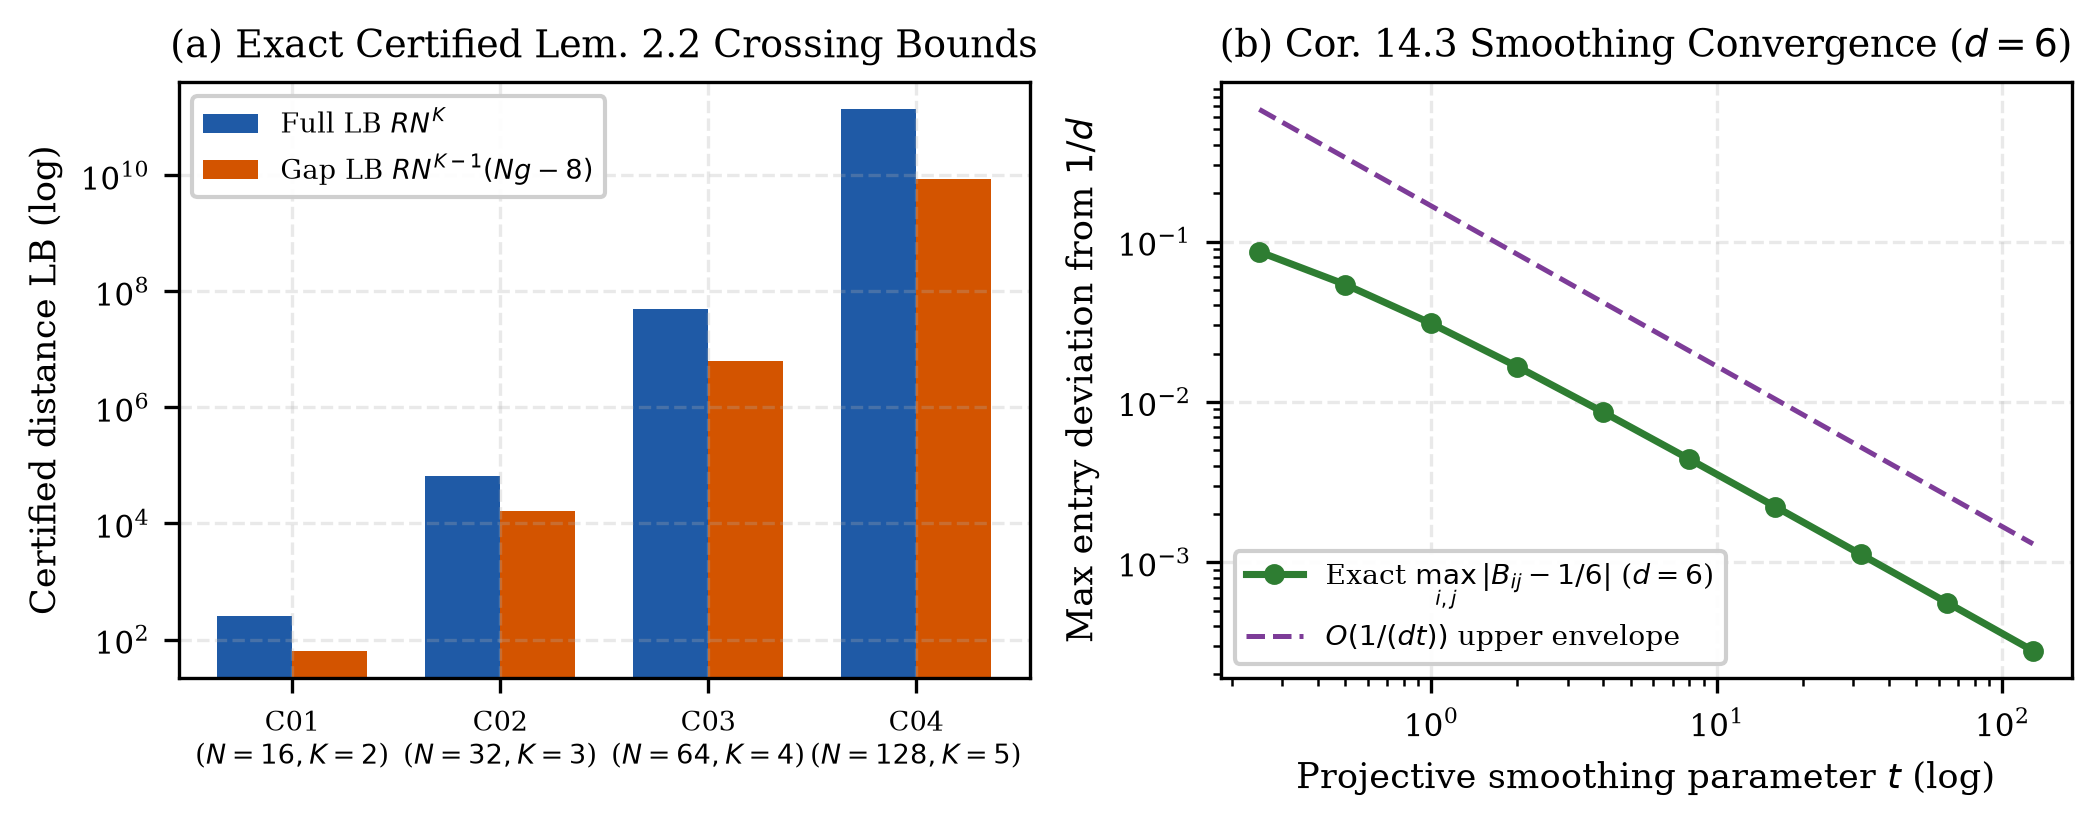
\includegraphics[width=\columnwidth]{figures/fig1_crossing_and_smoothing.png}
\vspace{-1.3em}
\caption{\textbf{(a)}~Exact certified Mode~1 Lemma~2.2 full distance LB $RN^K$ vs.\ gap distance LB $RN^{K-1}(Ng-8)$ across \texttt{C01}--\texttt{C04}. \textbf{(b)}~Exact rational Corollary~14.3 Stage-2 smoothing deviation $\max_{i,j}|B_{ij}-1/6|$ across $t\in[1/4,128]$ ($d=6$).}
\label{fig:cross}
\end{figure}

\begin{figure}[t]
\centering
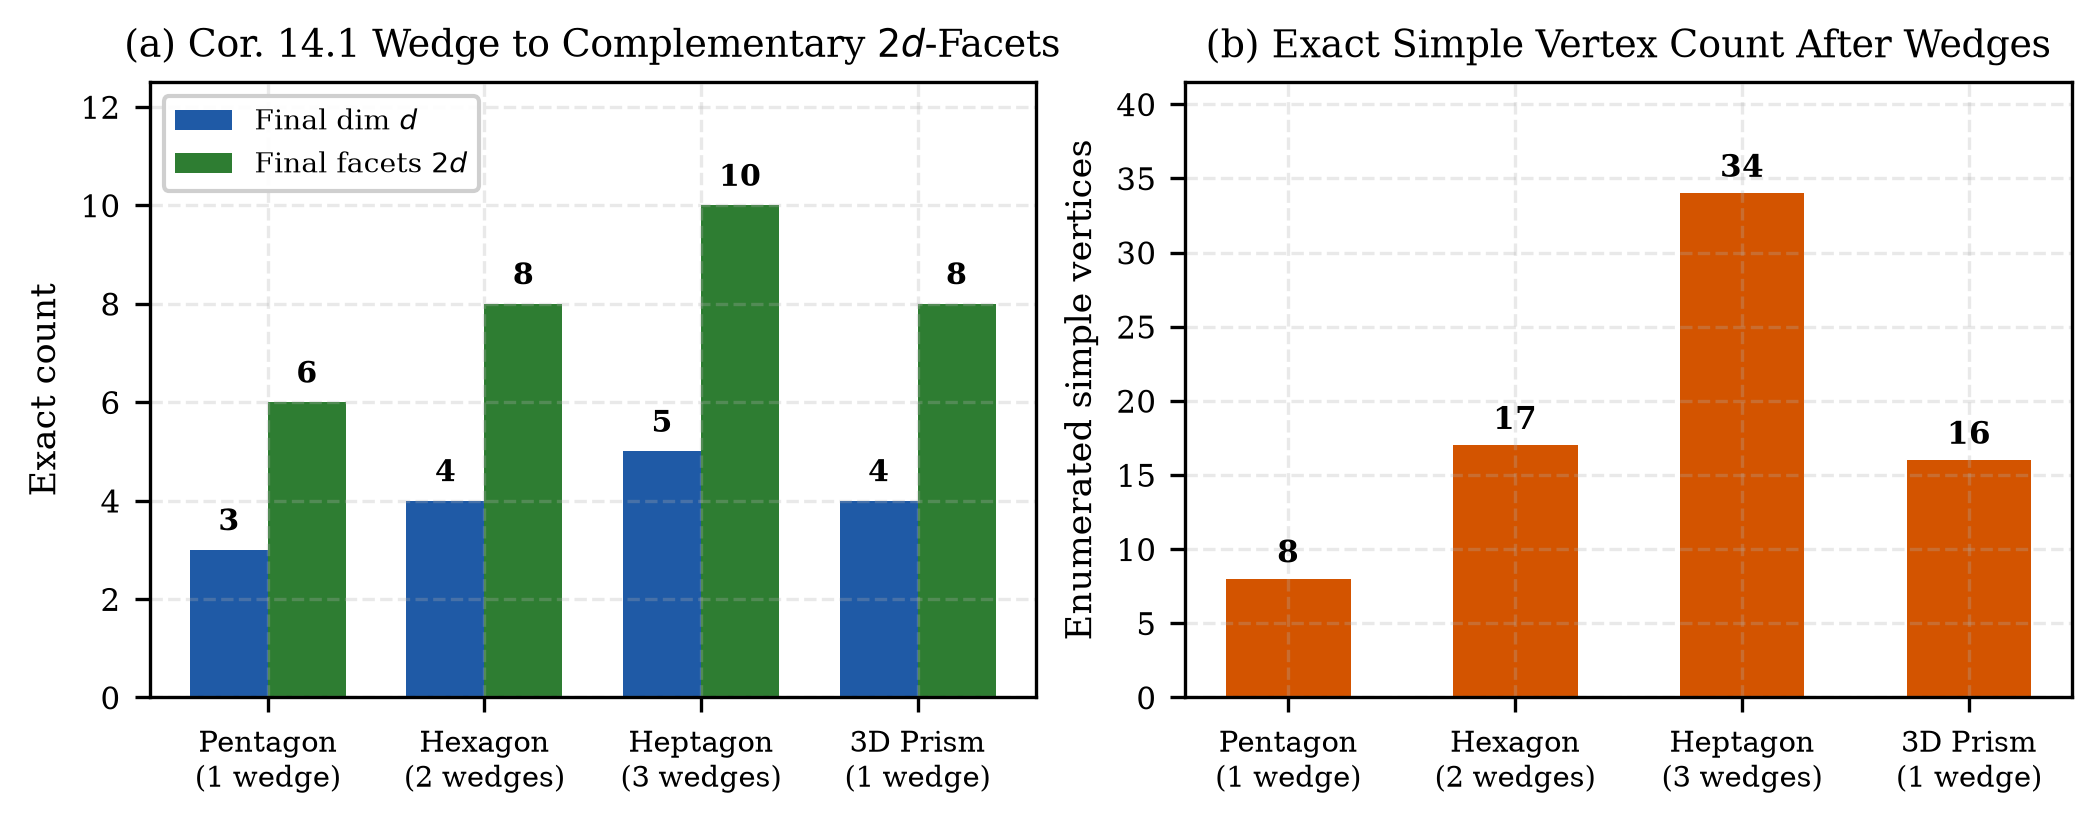
\includegraphics[width=\columnwidth]{figures/fig2_wedge_progression.png}
\vspace{-1.3em}
\caption{\textbf{(a)}~Exact Corollary~14.1 Klee--Walkup wedge progression to complementary $(d,2d)$ polytopes across pentagon (1 wedge), hexagon (2 wedges), heptagon (3 wedges), and 3D pentagonal prism (1 wedge). \textbf{(b)}~Exact enumerated simple vertex counts after wedging ($8, 17, 34, 16$).}
\label{fig:wedge}
\end{figure}

\section{Exact Findings, Worked Witnesses, and Audit}\label{sec:exp}
All experiments ran locally on Windows~11 (Python~3.12.6, Lean~4.35.0; 7-run means after warm-up).

\paragraph{1. Exact Wedge Lattices, Antiprism Widths \& Smoothing (Figs.~\ref{fig:cross}--\ref{fig:wedge}).}
Exact rational Klee--Walkup wedging lifts a 2D pentagon (5 facets, 1 wedge), hexagon (6 facets, 2 wedges), heptagon (7 facets, 3 wedges), and 3D pentagonal prism (7 facets, 1 wedge) to bounded simple complementary polytopes with (dimension, facet) pairs $(3,6)$, $(4,8)$, $(5,10)$, and $(4,8)$ and exactly $8, 17, 34,$ and $16$ enumerated simple vertices respectively. For Mode~3, exact dual-graph ridge-adjacency BFS certifies true widths $D_1=2$ (3D prism, 3 lateral facets) and $D_1=d\in\{3,4,5\}$ across our 3D, 4D, and 5D simplicial antiprisms ($6, 14, 30$ lateral facets). For Corollary~14.3's Stage-2 smoothing at $d=6$, $\max_{i,j}|B_{ij}-1/6|$ decays monotonically from $233/2700$ at $t=1/4$ to $233/830520$ at $t=128$.

\begin{figure}[t]
\centering
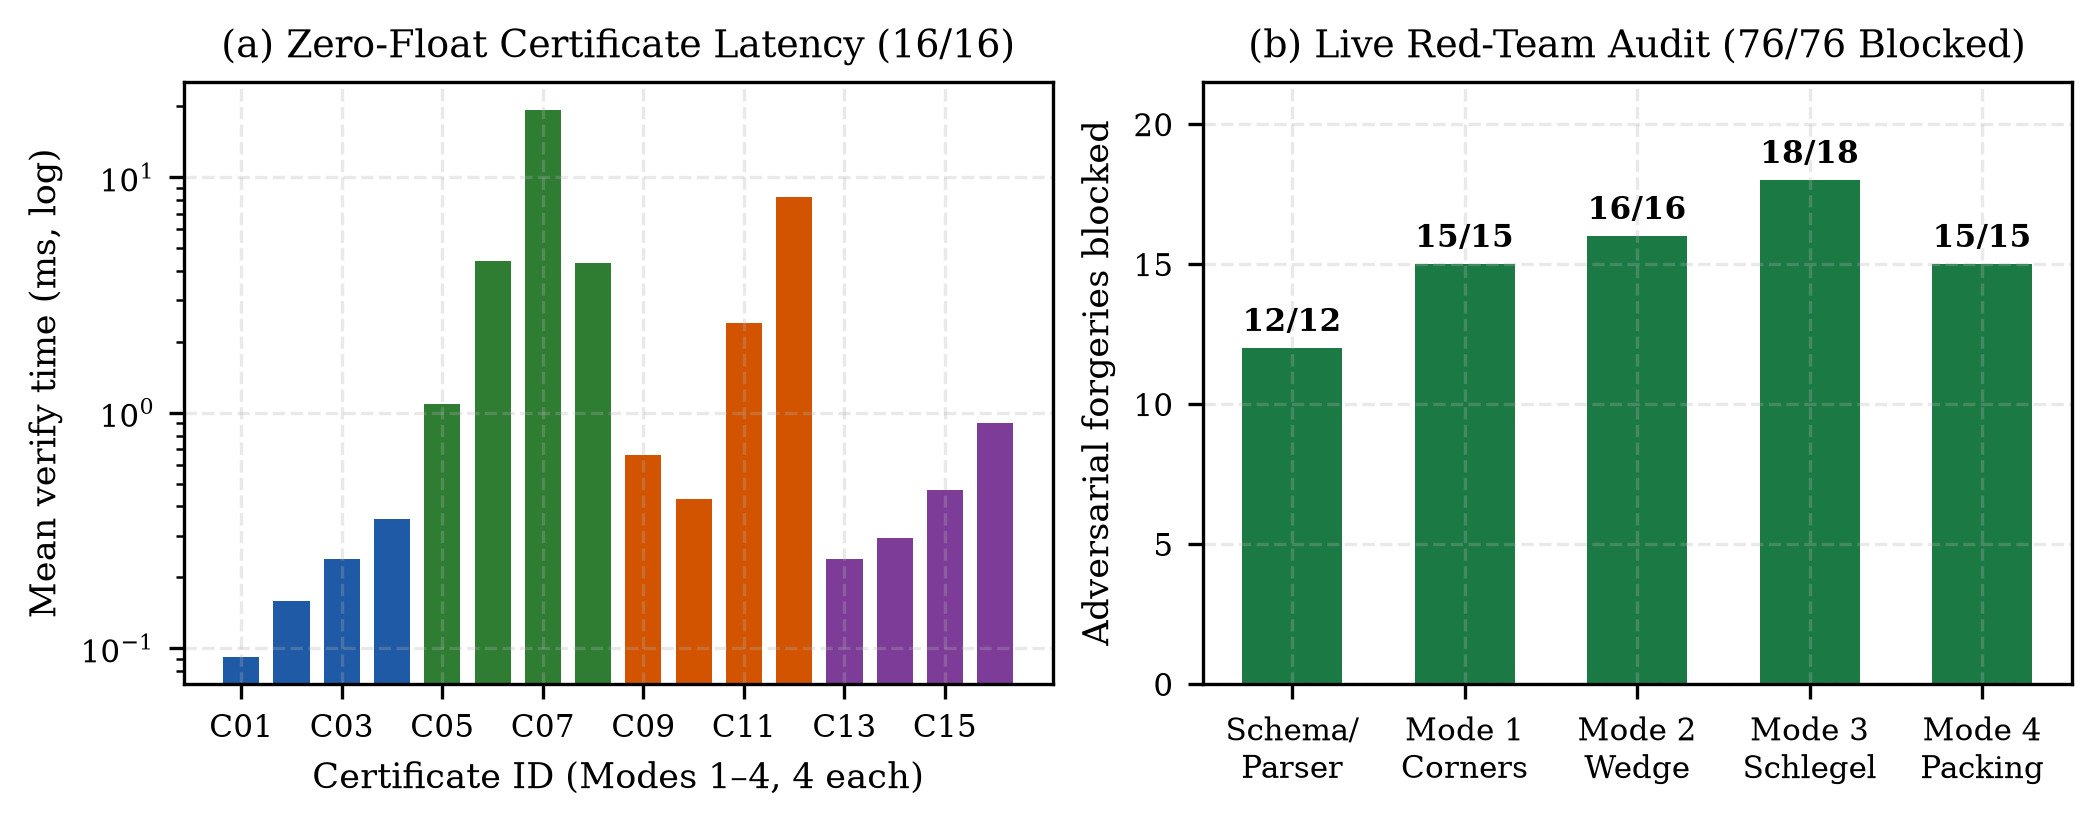
\includegraphics[width=\columnwidth]{figures/fig3_atlas_and_redteam.png}
\vspace{-1.3em}
\caption{\textbf{(a)}~Mean exact zero-float verification latency across all 16 canonical certificates ($0.092$--$19.354\,\mathrm{ms}$, log scale). \textbf{(b)}~Live adversarial red-team audit rejecting 76/76 forgeries across five attack classes with exact error-branch assertions.}
\label{fig:atlas}
\end{figure}

\noindent\textbf{2. Hand-Verifiable Worked Exact Witnesses (One per Mode).}\nopagebreak
\begin{itemize}[leftmargin=1.2em,itemsep=1pt,topsep=2pt]
  \item \textbf{Mode~1 (\texttt{C01}, 3 V-corners at $x\in\{1,3,5\}$, $N{=}16,K{=}2,R{=}1,g{=}3/4$):} The 7-waypoint rational zigzag satisfies $z\ge\min_k|x-a_k|$ everywhere and attains $z=0$ at all 3 corners with slopes $\pm 2$ (5 exact interior bends), certifying $R N^K=256$, gap bound $1\cdot 16\cdot(12-8)=64$, and Theorem~1.2 padding $(d_0,f_0)=(4,8)\to (20,40)$.
  \item \textbf{Mode~2 (\texttt{C05}, 2D pentagon $\to$ 3D wedge):} Starting from $x\ge 0, y\ge 0, x\le 2, y\le 2, x+y\le 3$ with disjoint tips $(0,0)$ and $(2,1)$, wedging the sole uncovered facet $y\le 2$ produces a bounded 3D simple 6-facet polytope with 8 enumerated vertices and complementary lifted tips $(0,0,0)$ and $(2,1,1)$.
  \item \textbf{Mode~3 (\texttt{C09}, Fig.~7 triangular antiprism):} With $U=\{(1,0),(0,1),(-1,-1)\}$ ($0\in\mathrm{int}(\mathrm{conv}(U))$) and $V=-\frac{1}{2}U$, $(U+V)/2$ yields 9 exact pairwise sums, all 6 lateral facets have rank $2$ and $b+c\in\{1,7/2\}>0$, and exact dual BFS certifies true width $D_1=3$ (section distance $1$, Schlegel depth $2$).
  \item \textbf{Mode~4 (\texttt{C13}, $k{=}2\to d{=}4$, $M{=}2,t{=}5$):} From nonnegative $A=\bigl(\begin{smallmatrix}3/4&1/4\\1/5&4/5\end{smallmatrix}\bigr)$, Stage~1 yields $c=(\frac{61}{40},\frac{59}{40})$, $h=4$, doubly-stochastic $B_0$ verified on $x=(\frac{1}{2},\frac{1}{3})$, and Stage~2 yields $4\times 4$ symmetric invertible doubly-stochastic $B$ with exact $\max|B_{ij}-1/4|=17/1120 < 1/20$.
\end{itemize}

\begin{table}[t]
\centering
\caption{Canonical 16-certificate \texttt{HIRSCH-DIAM-CERT-1.0} atlas (\texttt{exp1\_certificate\_atlas.json}; all 16 verified).}
\label{tab:atlas}
\scriptsize
\setlength{\tabcolsep}{1.8pt}
\resizebox{\columnwidth}{!}{%
\begin{tabular}{@{}c l c l r@{}}
\toprule
ID & Certificate Name & M & Exact Certified Witness Summary & ms \\
\midrule
C01 & \texttt{m1\_corners\_3\_n16\_k2} & M1 & 3 corners (5 breaks), $N^K{=}256$, gap $64$ & 0.092 \\
C02 & \texttt{m1\_corners\_5\_n32\_k3} & M1 & 5 corners (9 breaks), $2N^K{=}65536$, gap $16384$ & 0.159 \\
C03 & \texttt{m1\_corners\_7\_n64\_k4} & M1 & 7 corners (13 breaks), $3N^K{=}5.03{\times}10^7$ & 0.239 \\
C04 & \texttt{m1\_corners\_9\_n128\_k5} & M1 & 9 corners (17 breaks), $4N^K{=}1.37{\times}10^{11}$ & 0.355 \\
C05 & \texttt{m2\_wedge\_pentagon\_2d\_to\_3d} & M2 & 2D/5f $\xrightarrow{1\text{w}}$ 3D/6f, 8 simple verts & 1.091 \\
C06 & \texttt{m2\_wedge\_hexagon\_2d\_to\_4d} & M2 & 2D/6f $\xrightarrow{2\text{w}}$ 4D/8f, 17 simple verts & 4.404 \\
C07 & \texttt{m2\_wedge\_heptagon\_2d\_to\_5d} & M2 & 2D/7f $\xrightarrow{3\text{w}}$ 5D/10f, 34 simple verts & 19.354 \\
C08 & \texttt{m2\_wedge\_prism\_3d\_to\_4d} & M2 & 3D/7f $\xrightarrow{1\text{w}}$ 4D/8f, 16 simple verts & 4.341 \\
C09 & \texttt{m3\_schlegel\_antiprism\_3d\_fig7} & M3 & 3D antiprism (6f), 9 sums, $D_1{=}3\to(1,2)$ & 0.660 \\
C10 & \texttt{m3\_schlegel\_prism\_3d} & M3 & 3D prism (3f), 6 sums, $D_1{=}2\to(0,1)$ & 0.430 \\
C11 & \texttt{m3\_schlegel\_antiprism\_4d} & M3 & 4D antiprism (14f), 16 sums, $D_1{=}4\to(2,3)$ & 2.407 \\
C12 & \texttt{m3\_schlegel\_antiprism\_5d} & M3 & 5D antiprism (30f), 25 sums, $D_1{=}5\to(3,4)$ & 8.263 \\
C13 & \texttt{m4\_packing\_k2\_even\_d4} & M4 & $k{=}2\to d{=}4$: $\max|B_{ij}{-}\frac{1}{4}|{=}17/1120$ & 0.239 \\
C14 & \texttt{m4\_packing\_k2\_odd\_d5} & M4 & $k{=}2\to d{=}5$: $\max|B_{ij}{-}\frac{1}{5}|{=}4/255$ & 0.295 \\
C15 & \texttt{m4\_packing\_k3\_even\_d6} & M4 & $k{=}3\to d{=}6$: $\max|B_{ij}{-}\frac{1}{6}|{=}233/130680$ & 0.471 \\
C16 & \texttt{m4\_packing\_k4\_odd\_d9} & M4 & $k{=}4\to d{=}9$: $\max|B_{ij}{-}\frac{1}{9}|{=}8/4059$ & 0.905 \\
\bottomrule
\end{tabular}}
\end{table}

\paragraph{3. 16-Certificate Atlas \& 82-Test Red-Team Audit (Table~\ref{tab:atlas}, Fig.~\ref{fig:atlas}).}
Table~\ref{tab:atlas} lists all 16 canonical certificates verified in $0.092$--$19.354\,\mathrm{ms}$. \texttt{tests/test\_\allowbreak suite.py} runs 82 pytest checks: 1 full 16-certificate replay, 3 raw-JSON parser guards (float, \texttt{NaN}, duplicate keys), 2 exact regressions (Corollary~14.3 Stage-2 symmetry/invertibility and 4D hexagon wedge counts), and 76 parametrized live adversarial forgeries (12 schema/parser, 15 Mode~1, 16 Mode~2, 18 Mode~3, 15 Mode~4), each asserting an exact regex on its intended \texttt{CertificateError} branch. \texttt{scripts/verify\_\allowbreak all.py} enforces all 5 gates including strict axiom whitelisting and a 41-file SHA-256 manifest.

\section{Conclusion}\label{sec:conc}
We built an independent, explicitly scoped, zero-floating-point verification companion for the discrete convex-corner, product-padding, bounded Klee--Walkup wedge, complete Schlegel prismatoid/middle-section, and two-stage symmetric doubly-stochastic packing mechanisms of OpenAI's superpolynomial polytope diameter preprint~\cite{openai2026hirsch}, pairing 18 constructive Lean~4.35.0 sub-lemmas (zero \texttt{sorry}, zero \texttt{Classical.choice}) with the pure-\texttt{int}/\texttt{Fraction} 4-mode auditor \texttt{HIRSCH-\allowbreak DIAM-\allowbreak CERT-1.0}, 16 canonical exact finite witnesses, and 76/76 live adversarial forgery rejections.

{\footnotesize
\bibliographystyle{plain}
\bibliography{references}}
\end{document}
